\documentclass[]{article}

% Imports the catppuccin theme, using the mocha flavor,
% from the directory above. Actual implementation
% wouldn't need the import package unless the theme
% and the document are in different directories.
\usepackage{import}
\usepackage{xcolor}
% \usepackage{fancyhdr}
\usepackage{cancel}
\usepackage{mathtools}

% For permutations and combinations
\newcommand\Myperm[2][^n]{\prescript{#1\mkern-2.5mu}{}P_{#2}}
\newcommand\Mycomb[2]{\prescript{#1\mkern-0.5mu}{}C_{#2}}

% Colors
\definecolor{yorhabg}{HTML}{FFFFFF}
\definecolor{yorhafg}{HTML}{000000}
\definecolor{yorhagrid}{HTML}{B5AF9C}
\definecolor{mred}{HTML}{D67069}
\definecolor{mblue}{HTML}{6887A1}

\pagecolor{yorhabg}
\color{yorhafg}

\usepackage{preamble}

% Removes padding above title
\usepackage{titling}
\setlength{\droptitle}{-10em}

% Font package
\usepackage[T1]{fontenc}

\usepackage{fouriernc}

\usepackage{sectsty}
\usepackage{graphicx}
\usepackage{amsmath}
\usepackage{amsfonts}
\usepackage{amssymb}
\usepackage[skins, most]{tcolorbox}
\usepackage{enumitem}

\DeclareMathOperator{\sgn}{sgn}

\usepackage{tikz}
\usepackage{eso-pic}
\usetikzlibrary{calc,shadows.blur}
\usetikzlibrary{angles, quotes}
\usetikzlibrary{3d}

% Margins
\topmargin=0in
\evensidemargin=0in
\oddsidemargin=0in
\textwidth=6.5in
\textheight=9.0in
\headsep=0.25in

\AtBeginEnvironment{tcolorbox}{\small}

\newtcolorbox{imp}{enhanced,arc=0mm,colback=yorhabg,colframe=mred,leftrule=10mm,coltext=yorhafg,%
overlay={\node[anchor=west,outer sep=2pt] at (frame.west) {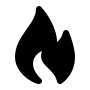
\includegraphics[width=6mm]{images/imageb.png}}; }}

\newtcolorbox{shortcut}{enhanced,arc=0mm,colback=yorhabg,colframe=mred,leftrule=10mm,coltext=yorhafg, coltitle=yorhabg, title=\texttt{Shortcut.}, 
overlay={\node[anchor=west,outer sep=2pt] at (frame.west) {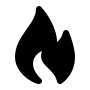
\includegraphics[width=6mm]{images/imageb.png}}; }}

\newtcolorbox{question}[1]{
    enhanced, 
    colback=yorhabg,
    colframe=mblue,
    coltext=yorhafg,
    coltitle=yorhabg,
    attach boxed title to top left={yshift*=-\tcboxedtitleheight}, 
    title=\texttt{#1},
    boxed title size=title,
    boxed title style={%
        rounded corners=northeast, 
        rounded corners=northwest, 
        colback=tcbcolframe, 
        boxrule=0pt,
    },
    underlay boxed title={%
        \path[fill=tcbcolframe] (title.south west)--(title.south east) 
            to[out=0, in=180] ([xshift=5mm]title.east)--
            (title.center-|frame.east)
            [rounded corners=5pt] |- 
            (frame.north) -| cycle; 
    },
}

\newcommand\bb[1]{\textcolor{yorhafg}{\textbf{#1}}}

\title{\textbf{CSCA67 - Assignment \#2}}
\author{Satyajit Datta \ 1012033336}
\date{\today}

\begin{document}
\maketitle

\section{Quantifiers}
For each of the following logical expressions, write a corresponding (English) mathematical statement, indicate
whether the statement is true or false, and provide a brief explanation. Universe of discourse is $\mathbb{R}$, the real numbers.

\begin{question}{1.1}
\[
\exists x \forall y,\; x + y = y
\]
\end{question}
\begin{enumerate}[label=(\alph*)]
    \item \textbf{English statement:} There exists a real number $x$ such that for all $y \in \mathbb{R}$, $x + y = y$.
    \item \textbf{Truth value:} True.
    \item \textbf{Explanation:} Let $x = 0$. Then $x + y = y$ for all $y$.
\end{enumerate}

\begin{question}{1.2}
\[
\forall x\forall y,\;((x \ne 0) \land (y \ne 0)) \leftrightarrow (xy \ne 0)
\]
\end{question}
\begin{enumerate}[label=(\alph*)]
    \item \textbf{English statement:}
    \item \textbf{Truth value:}
    \item \textbf{Explanation:}
\end{enumerate}

\begin{question}{1.3}
\[
\forall x\exists y,\; x^2 = y
\]
\end{question}
\begin{enumerate}[label=(\alph*)]
    \item \textbf{English statement:}
    \item \textbf{Truth value:}
    \item \textbf{Explanation:}
\end{enumerate}

\begin{question}{1.4}
\[
\exists x\forall y,\; xy = 0
\]
\end{question}
\begin{enumerate}[label=(\alph*)]
    \item \textbf{English statement:}
    \item \textbf{Truth value:}
    \item \textbf{Explanation:}
\end{enumerate}

\begin{question}{1.5}
\[
\exists x \exists y,\; x + y\ne y +x
\]
\end{question}
\begin{enumerate}[label=(\alph*)]
    \item \textbf{English statement:}
    \item \textbf{Truth value:}
    \item \textbf{Explanation:}
\end{enumerate}

\begin{question}{1.6}
\[
\exists x \forall y,\; (y \ne 0) \rightarrow (xy = 1)
\]
\end{question}
\begin{enumerate}[label=(\alph*)]
    \item \textbf{English statement:}
    \item \textbf{Truth value:}
    \item \textbf{Explanation:}
\end{enumerate}

\begin{question}{1.7}
\[
\forall y \exists x,\; (y \ne 0) \rightarrow (xy = 1)
\]
\end{question}
\begin{enumerate}[label=(\alph*)]
    \item \textbf{English statement:}
    \item \textbf{Truth value:}
    \item \textbf{Explanation:}
\end{enumerate}

\begin{question}{1.8}
\[
\forall x\forall y,\; ((x \ge 0) \land (y \ge 0)) \rightarrow \exists z, 0 \le x \le z \le y
\]
\end{question}
\begin{enumerate}[label=(\alph*)]
    \item \textbf{English statement:}
    \item \textbf{Truth value:}
    \item \textbf{Explanation:}
\end{enumerate}

\begin{question}{1.9}
\[
\forall x\forall y, (x \ge 0) \rightarrow ((y \rightarrow 0) \rightarrow ( x + y \ge 0))
\]
\end{question}
\begin{enumerate}[label=(\alph*)]
    \item \textbf{English statement:}
    \item \textbf{Truth value:}
    \item \textbf{Explanation:}
\end{enumerate}

\begin{question}{1.10}
\[
\forall x\forall y,\; ((x \ge 0) \land (y \ge 0)) \leftrightarrow (xy \ge 0)
\]
\end{question}
\begin{enumerate}[label=(\alph*)]
    \item \textbf{English statement:}
    \item \textbf{Truth value:}
    \item \textbf{Explanation:}
\end{enumerate}
\section{Negation}
For each of the following sentences:
\begin{enumerate}[label=(\alph*)]
  \item Write a logical expression that represents the English sentence.
  \item Write an English sentence that is the negation of the original sentence.
  \item Negate the expression in Step 1, and use logical equivalence rules to
  demonstrate that the result is equivalent to the logical form of the English sentence in Step 2.
\end{enumerate}

$M(x)$ stands for “$x$ is a Mathematics student”, $C(x)$ stands for “$x$ is a Computer Science student”, $S(x)$ stands
for “$x$ is a Statistics student”, $T(x, y)$ stands for “student $x$ takes course $y$” (“student $x$ is in course $y$”), $D(x)$ stands
for “$x$ is a discrete mathematics class”, $P(x)$ stands for “$x$ is a programming class”, and $L(x)$ stands for “$x$ is a
Political Science class”. Universe of discourse is students and classes. 

Do not use the shortcut $\exists!x$ in any of your solutions.
\begin{question}{2.1}
Everyone in any discrete mathematics class is either a Mathematics student, a Computer Science student, or a Statistics student.
\end{question}
\begin{enumerate}[label=(\alph*)]
    \item \textbf{Logical Expression:}
    \item \textbf{English sentence:}
    \item \textbf{Explanation:}
\end{enumerate}

\begin{question}{2.2}
Only Computer Science students take programming classes.
\end{question}
\begin{enumerate}[label=(\alph*)]
    \item \textbf{Logical Expression:}
    \item \textbf{English sentence:}
    \item \textbf{Explanation:}
\end{enumerate}

\begin{question}{2.3}
Non-Mathematics students take no more than two discrete mathematics classes.
\end{question}
\begin{enumerate}[label=(\alph*)]
    \item \textbf{Logical Expression:}
    \item \textbf{English sentence:}
    \item \textbf{Explanation:}
\end{enumerate}

\begin{question}{2.4}
There is at least one Statistics student who takes a discrete mathematics class, a political science class, and no
programming classes.
\end{question}
\begin{enumerate}[label=(\alph*)]
    \item \textbf{Logical Expression:}
    \item \textbf{English sentence:}
    \item \textbf{Explanation:}
\end{enumerate}

\begin{question}{2.5}
At least two Computer Science students take a Political Science class.
\end{question}
\begin{enumerate}[label=(\alph*)]
    \item \textbf{Logical Expression:}
    \item \textbf{English sentence:}
    \item \textbf{Explanation:}
\end{enumerate}

\section{Deductive Reasoning}
\section{Operations on Sets}
\section{Quantifiers and Sets}
\section{Quantifiers and Logical Equivalence}


\end{document}